\documentclass{article}
\usepackage[utf8]{inputenc}
\usepackage{titling}
\usepackage{graphicx}
\usepackage{xcolor}
\usepackage[colorlinks=true,linkcolor=darkgray, urlcolor =gray]{hyperref}
\usepackage[spanish]{babel}
\DeclareUnicodeCharacter{301}{~}
\usepackage{url}
\usepackage{graphicx}
\usepackage{caption}
\usepackage{subcaption}
\DeclareUnicodeCharacter{202F}{\,}


\title{Gestión documental con Alfresco}
\author{Grupo O\\Álvaro Fernández Palma\\ Alina Altynguzhina\\ Iman Hasnaouia Meskini\\ Cristina Díaz García}
\date{Enero 2019}

\renewcommand\maketitlehooka{\null\mbox{}\vfill}
\renewcommand\maketitlehookd{\vfill\null}


\begin{document}

\addcontentsline{toc}{section}{Índice general}

\begin{titlingpage}
\maketitle

\begin{center}

\includegraphics[scale=0.4]{images/alfresco.jpg} 
\end{center}

\end{titlingpage}

\newpage

\tableofcontents

\newpage

\section{Introducción}

Alfresco es una herramienta tipo DMS que es un sistema que se utiliza para seguir, gestionar y alojar documentos. 

\subsection{Objetivos de la Práctica}

Los objetivos de esta quinta práctica de la asignatura son afianzar los conceptos teóricos sobre Gestión Documental, Archivo Electrónico y Flujos de Trabajo usando la herramienta de Gestión Documental Alfresco. Esta práctica también nos permite afianzar otros conocimientos básicos previamente aprendidos en la asignatura, como posibilidades de integración y también, como en todas las prácticas, se mejora la habilidad de creación de informes. Y poder colaborar entre los compañeros en un trabajo de forma más consistente controlando versiones, asignando tareas.

\subsection{Funcionalidad de Alfresco}

Alfresco es un sistema de administración de contenidos de código fuente libre distribuido en tres variantes: Afresco Community Edition (Software Libre), Alfresco Enterprise Edition (Software bajo licencia) y Alfresco Cloud Edition (SaaS). La plataforma de Alfresco dispone de distintas herramientas: Alfresco Content Services (ECM), Alfresco Process Services (BPM), Alfresco Governance Services (RM) y Alfresco Application Development Framework (ADF). En esta práctica utilizaremos la versión online de Alfresco Content Services (ECM), una herramienta que permite administrar contenidos de manera flexible creando flujos de trabajo, con herramientas de administración de procesos o tareas y posibilidad de integración con otros sitios o aplicaciones. En especial usaremos la herramienta de Alfresco Share, que es una interfaz de usuario para administradores. Es capaz de mantener un registro de diferentes versiones de documentos creados y modificados por diferentes usuarios, colecciona archivos e información en una estructura consistente, proporciona información a los usuarios distribuyendo de forma segura, es una herramienta colaborativa. 


\subsection{Reparto de Tareas}

\begin{center}
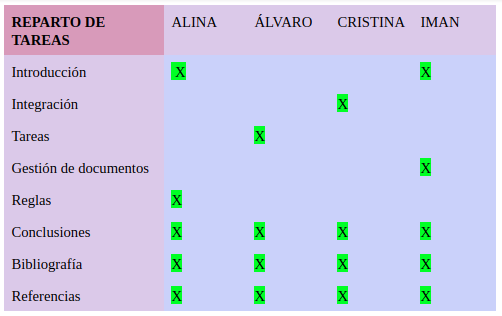
\includegraphics[scale=0.6]{images/tareas.png}
\end{center}

\section{Integración}

Alfresco es abierto y modular por diseño (en todos los niveles, incluido el repositorio, interfaz web, nube y aplicaciones móviles), y se integra muy bien con aplicaciones punteras. También da soporte a otro tipo de aplicaciones, y proporcionan APIs abiertas para las los desarrolladores de aplicaciones.

Al ser de código abierto y adaptarse a los estándares abiertos (incluidos CMIS, CIFS y WebDAV), su integración y personalización es genial para casi cualquier proyecto.  Su API es una API REST pública que permite una fácil personalización y automatización de procesos y su mantenimiento.

Alfresco también proporciona un Framework para desarrollo de aplicaciones que usa Angular para ofrecer una amplia variedad de componentes de servicios de contenido y proceso altamente configurables y reutilizables basados en el diseño de Angular Material.
Entre las aplicaciones punteras del sector se encuentran Salesforce, las aplicaciones de Google (Google Docs, Google Drive…), el paquete ofimático de Microsoft Office y Outlook, entre otras.

\section{Tareas}

Para llevar a cabo esta asignación en Alfresco previamente tendremos que tener dado de alta al menos un usuario, colaborador ó administrador del entorno de trabajo ya que dichas tareas irán basadas sobre los documentos que tengamos alojados en dicho entorno y estos deberán de ser supervisados, valorados y editados por las personas que tengan acceso a dicho workflow.

Podremos asignar tanto tareas en grupo como individuales, en éste ejemplo mostraremos una asignación de tarea para una única persona.

\begin{center}
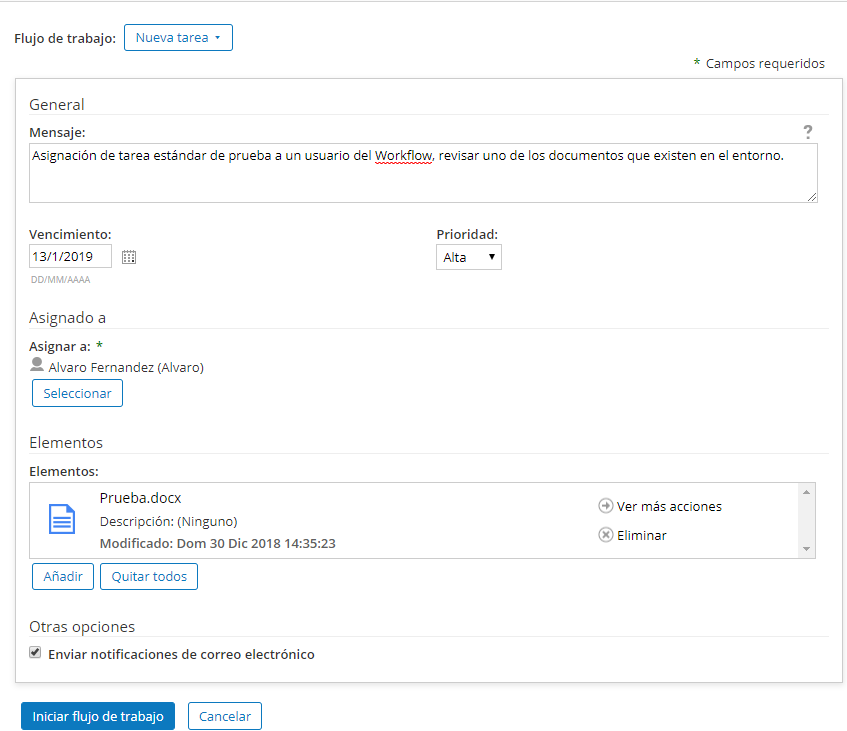
\includegraphics[scale=0.6]{images/task.png}
\end{center}

Para poder llegar a esta ventana tenemos que ir al apartado de tareas del header y clickar la segunda opción, una vez en esta nueva sección clicamos la opción de crear/asignar una nueva tarea.
Podremos indicar el contenido de muchos campos con el fin de informar a la persona encargada de realizar la tarea que estemos elaborando.
Primeramente podremos colocar un mensaje a modo de resumen de lo que consistirá la tarea, seguidamente indicaremos el nivel de prioridad y la fecha límite para realizar la tarea. A continuación se podrá elegir manualmente qué persona/grupo realizará dicha tarea (en tareas más complejas se pueden incluso añadir que en correcciones por grupo se ha de puntuar subjetivamente dicha tarea y, hasta que esta no alcance una nota media mínima, no se podrá aprobar para finalizarla)

Seguidamente podremos añadir cualquier elemento que veamos oportuno o necesario para la realización de dicha tarea, en éste caso, se necesita revisar un archivo contenido dentro de nuestro espacio de trabajo, así que lo añadiremos como elemento. Y finalmente podremos elegir si queremos que a dicha persona se le notifique por correo que se le ha asignado una nueva tarea.
Iniciamos el flujo de trabajo y, cuando la persona en cuestión desee visualizar/actualizar su tarea, esto es lo que verá:

\begin{center}
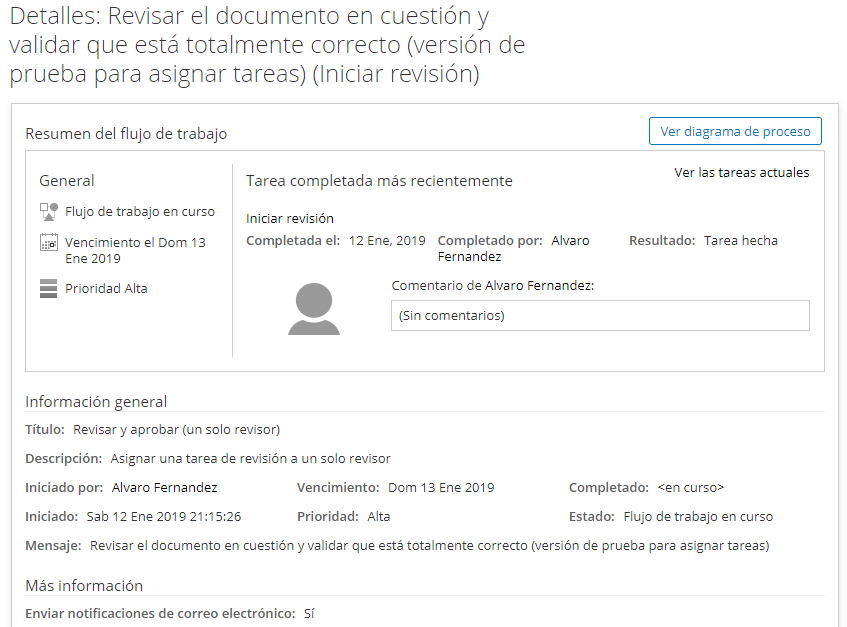
\includegraphics[scale=0.6]{images/diagrama.png}
\end{center}

Podremos ver el flujo de trabajo y la asignación de la tarea propiamente dicha, la información sobre la prioridad y la fecha límite de finalización, cuando se creó dicha tarea, si está finalizada, en curso, en proceso, etc. Si clicamos en "ver diagrama de proceso" en el botón superior derecho de la imagen veremos un pequeño diagrama explicativo de la situación actual de nuestra tarea

\begin{center}
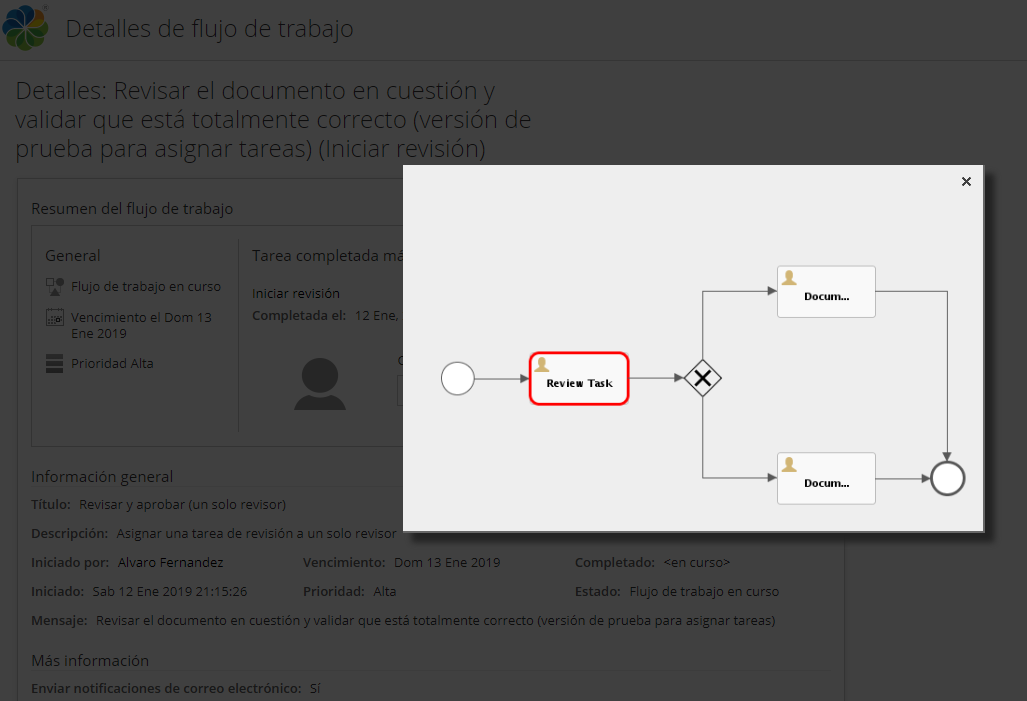
\includegraphics[scale=0.5]{images/flujo.png}
\end{center}

Donde podemos apreciar que nos encontramos en la fase inicial de dicha tarea. Ahora simplemente deberemos realizar una revisión de dicho documento que será señalizado como que dicho archivo forma parte de alguna tarea como elemento y, cuando la persona compruebe que está todo correcto, volverá a la pestaña de tareas y clickará ahora sí la primera opción "Mis tareas".

Podrá ver un listado de tareas asignadas (en este caso sólo hay 1) y podrá editar/actualizar el estado en el que se encuentren cada una de ellas.

Antes de realizar la tarea la persona en cuestión deberá "aceptar/aprobar" dicha tarea que se le ha sido encomendada, así pues entrará en la ventana de dicha tarea y clickará en la acción de editar (tiene el símbolo de un pincel cuando se hace hover sobre la celda de acciones).

\begin{center}
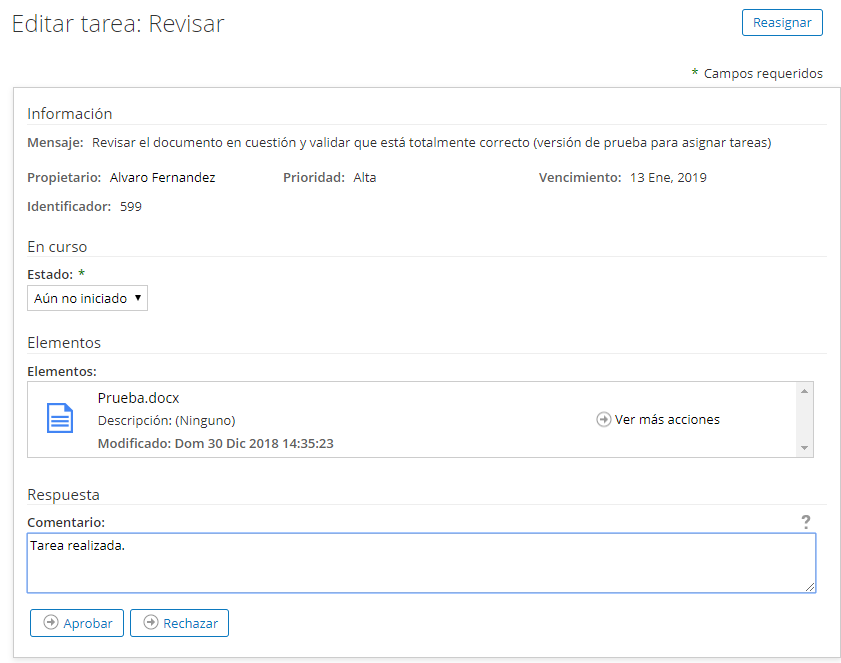
\includegraphics[scale=0.6]{images/revisar.png}
\end{center}

Ahora nuestro estado en el flujo de trabajo ha cambiado, porque ya hemos realizado una revisión subjetiva de lo que se pedía

\begin{center}
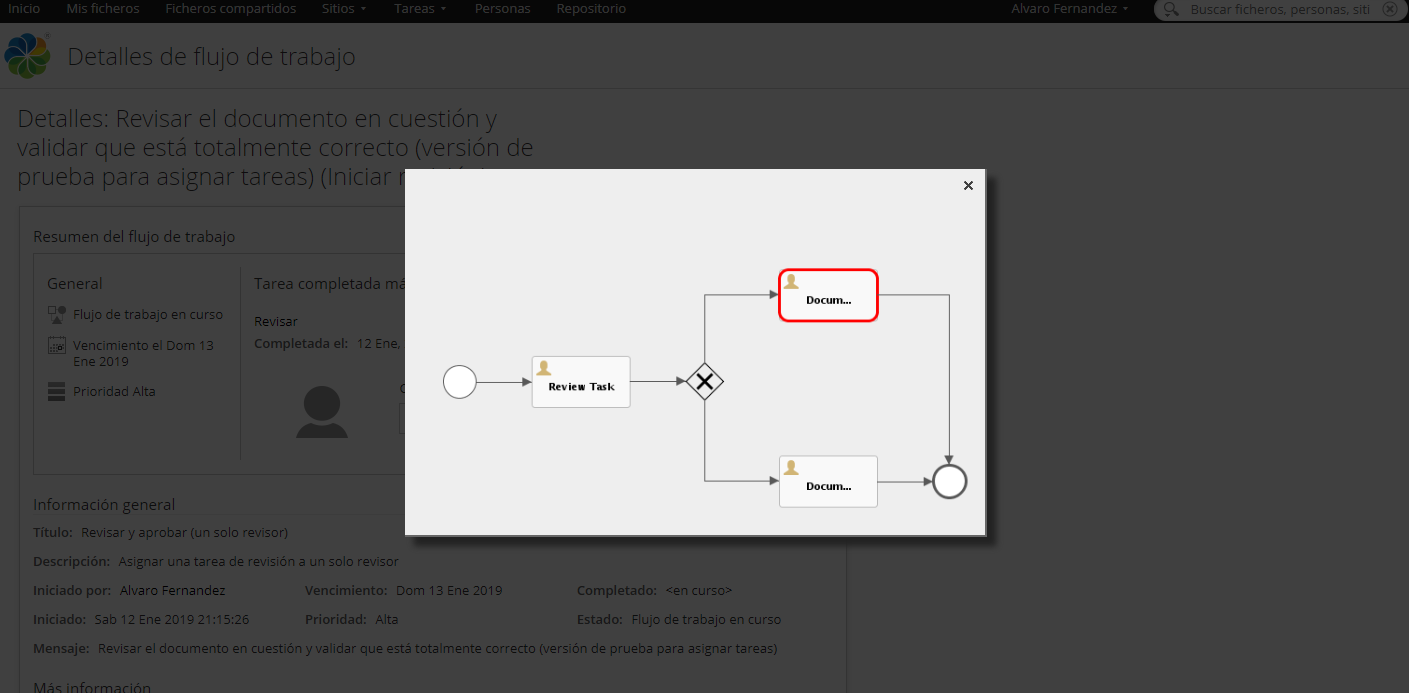
\includegraphics[scale=0.4]{images/flujo2.png}
\end{center}

En tareas actuales se vería reflejado la subtarea que aún queda pendiente para finalizar la tarea asignada y las que se hicieron previamente a ellas, en este caso, crear la tarea en cuestión.
Para actualizar la tarea, deberemos ir a la pestaña de "Acciones" y clicar sobre el pincel "editar".

\begin{center}
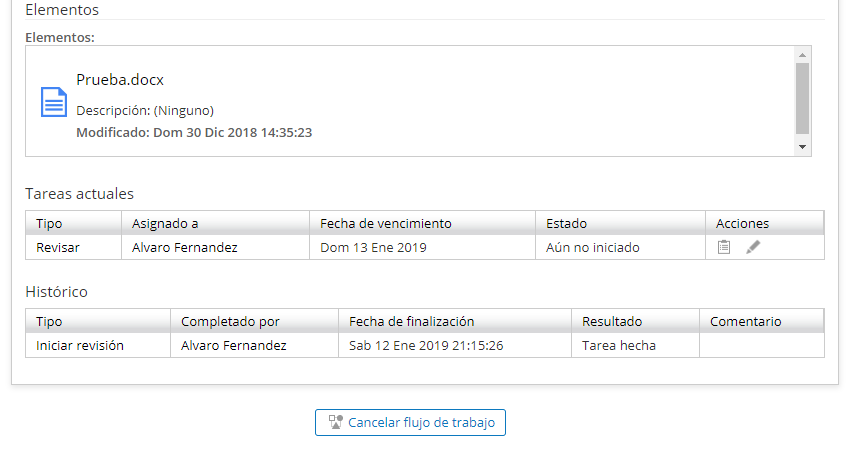
\includegraphics[scale=0.6]{images/editar.png}
\end{center}

Únicamente deberemos escribir algún comentarios si quisiéramos y, seguidamente clickar sobre el botón de tarea hecha y tanto la tarea como el flujo de trabajo llegaría a finalizar.

\begin{center}
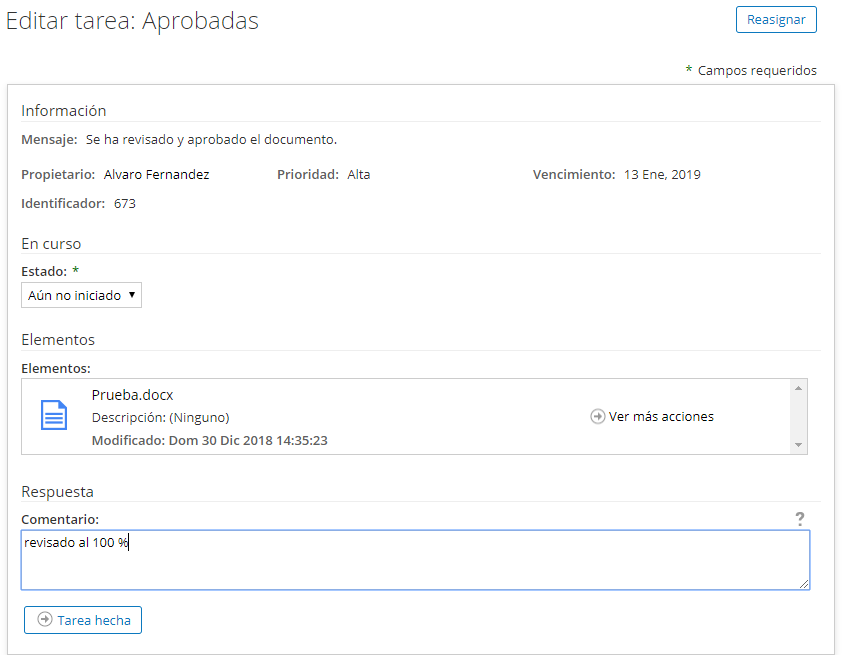
\includegraphics[scale=0.6]{images/aprobadas.png}
\end{center}

\section{Gestión de documentos}

\subsection{Creación de un espacio de trabajo}

Al acceder a la versión de prueba, automáticamente hay un espacio de trabajo creado con visibilidad pública. Nosotros crearemos un sitio llamado “Trabajando con documentos” con visibilidad privada.

\begin{center}
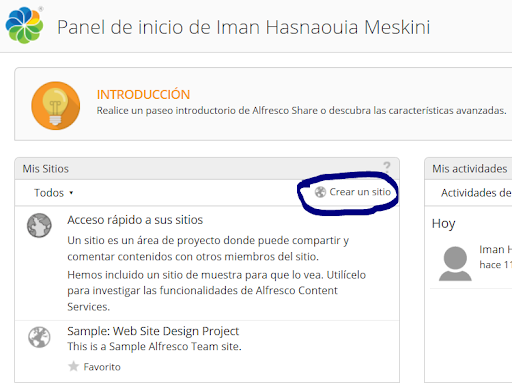
\includegraphics[scale=0.5]{images/workspace1.png}
\end{center}

\begin{center}
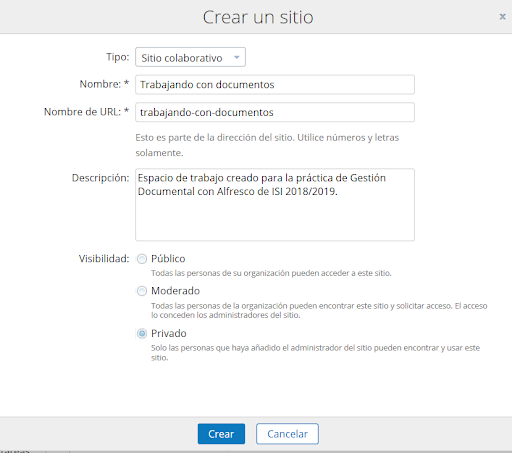
\includegraphics[scale=0.5]{images/workspace2.png}
\end{center}

\begin{center}
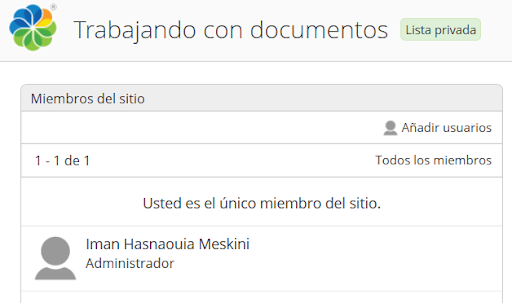
\includegraphics[scale=0.5]{images/workspace3.png}
\end{center}

Cuando se crea un nuevo sitio, se crea un espacio de trabajo vacío y la única persona que tiene acceso al sitio es el usuario que lo creó.

\subsection{Creación de usuarios}

Después de crear el espacio de trabajo o sitio nuevo, hemos creado un usuario para cada miembro del grupo, profesores y un usuario de prueba llamado “Test”. Para ello, se ha accedido a \textit{Herramientas de Administración y en Usuarios} y \textit{Grupos} se ha seleccionado \textit{Usuarios}. Allí para cada usuario se ha usado el nombre y el email correspondientes, y como contraseña se ha usado la cadena de caracteres “1234” por simplicidad.  Para acceder habría que pulsar \href{https://blctbt.trial.alfresco.com/share/page?mkt_tok=eyJpIjoiWXpRM05EbGpOamszWkRJeiIsInQiOiJSblJPbVFTVERZTnJhWHI5TGM4dHZXWkRHdmhlWlN0NlI0ZEQzZkgrc0ZiNElJaUo3K2k1a3RzOUh4UFNSaXU2RHlHTVVHYUhnblNGVFY0V1gyZlNZN0wxSk82anZudStVT1VKcWZqNVlGVlwvbUZmY01nRlVZVTRTZHRxbUZyeUUifQ\%3D\%3D}{este enlace} e introducir los datos necesarios para el login. Para los profesores, en vez de usar el email del campus, se ha usado una dirección de email ficticia, ya que la dirección de email de la UMA no es aceptada por la plataforma.

\begin{itemize}
\item Usuarios del grupo de Trabajo
\begin{figure}[h!]
        \begin{subfigure}[!]{0.25\textwidth} 
            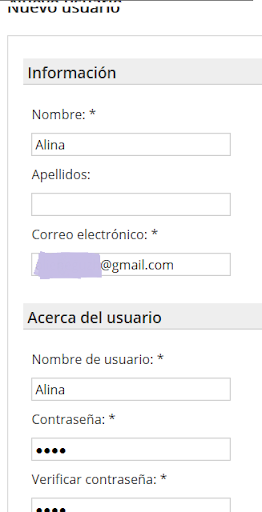
\includegraphics[width=\textwidth]{images/alina.png}
        \end{subfigure}       
        \begin{subfigure}[!]{0.25\textwidth} 
            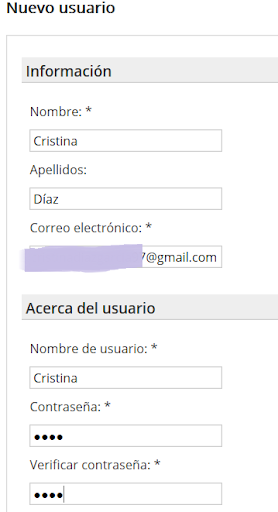
\includegraphics[width=\textwidth]{images/cristina.png}
        \end{subfigure}
        \begin{subfigure}[!]{0.25\textwidth} 
            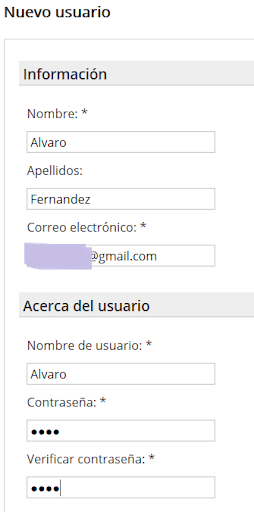
\includegraphics[width=\textwidth]{images/alvaro.png}
        \end{subfigure}
\end{figure}
\item Usuario de prueba
\begin{center}
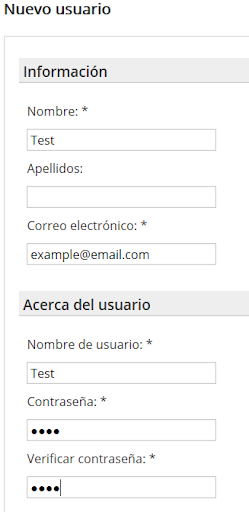
\includegraphics[scale=0.4]{images/test.png}
\end{center}
\item Usuario Profesores
\begin{center}
\begin{figure}[h!]
        \begin{subfigure}[!]{0.25\textwidth} 
            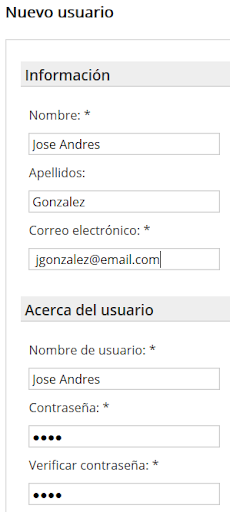
\includegraphics[width=\textwidth]{images/jose.png}
        \end{subfigure}       
        \begin{subfigure}[!]{0.25\textwidth} 
            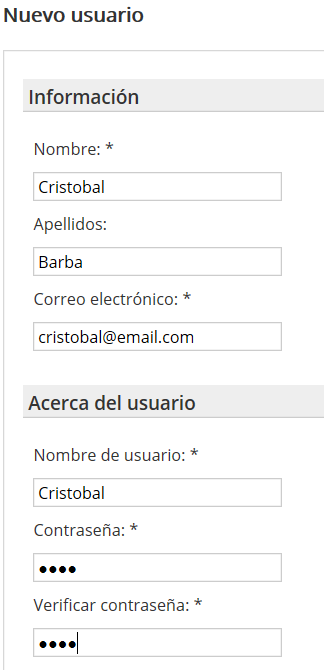
\includegraphics[width=\textwidth]{images/cristobal.png}
        \end{subfigure}
\end{figure}
\end{center}
\end{itemize}

Después de crear a todos los usuarios, hay que permitir a los usuarios acceder a nuestro nuevo espacio de trabajo o sitio y darles permisos de \textit{Colaborador}.

\begin{center}
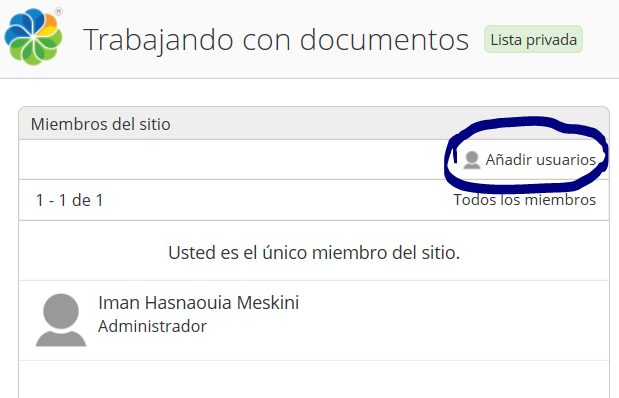
\includegraphics[scale=0.5]{images/adduser.png}
\end{center}

\begin{center}
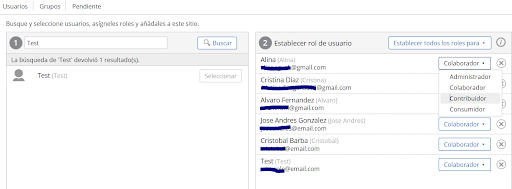
\includegraphics[scale=0.8]{images/adduser2.png}
\end{center}

\begin{center}
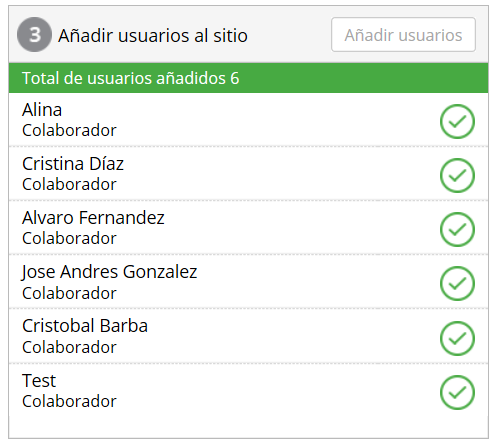
\includegraphics[scale=0.5]{images/adduser3.png}
\end{center} 

Tras realizar los tres pasos que se muestran en las imágenes anteriores, todos los usuarios tienen acceso al espacio de trabajo con permiso de Colaborador. Una vez que se entra a la página principal del sitio en Alfresco, se puede confirmar qué usuario tiene acceso y con qué rol:

\begin{center}
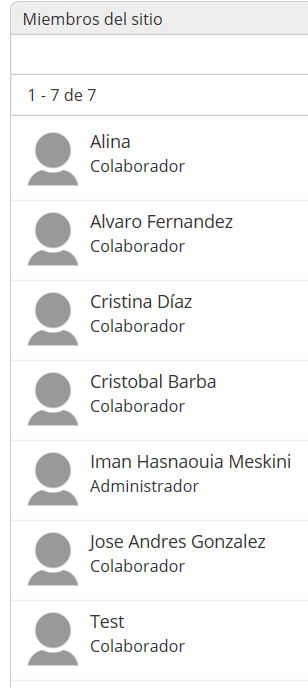
\includegraphics[scale=0.3]{images/roles.png}
\end{center} 

Y en el dashboard se muestra un panel de actividades que notifica de cualquier actividad realizada en el espacio de trabajo junto con el usuario que hizo la actividad.

\begin{center}
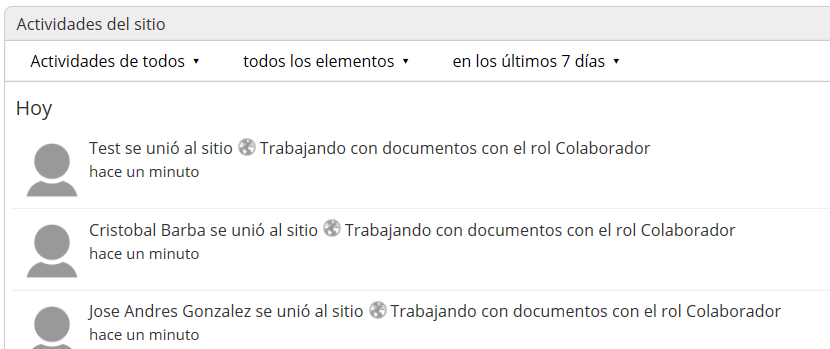
\includegraphics[scale=0.5]{images/activity.png}
\end{center}

\subsection{Permitir versionado del documento}

Para probar la funcionalidad de la gestión de documentos de Alfresco, vamos a acceder con el usuario Test, el cual es Colaborador, y desde ese usuario vamos a subir a la plataforma un documento de texto.

Primero iniciamos sesión:

\begin{center}
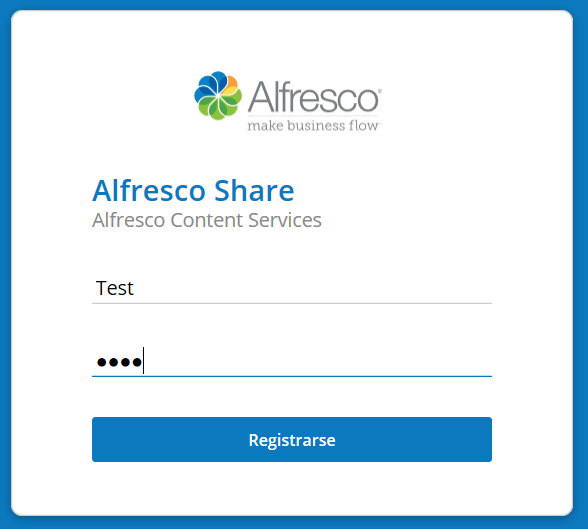
\includegraphics[scale=0.5]{images/session.png}
\end{center}

Si no hay ningún problema, después del inicio de sesión el usuario Test puede observar el dashboard completo y acceder al sitio. El usuario test accede a \textit{Biblioteca de Documentos} y carga el fichero.

\begin{center}
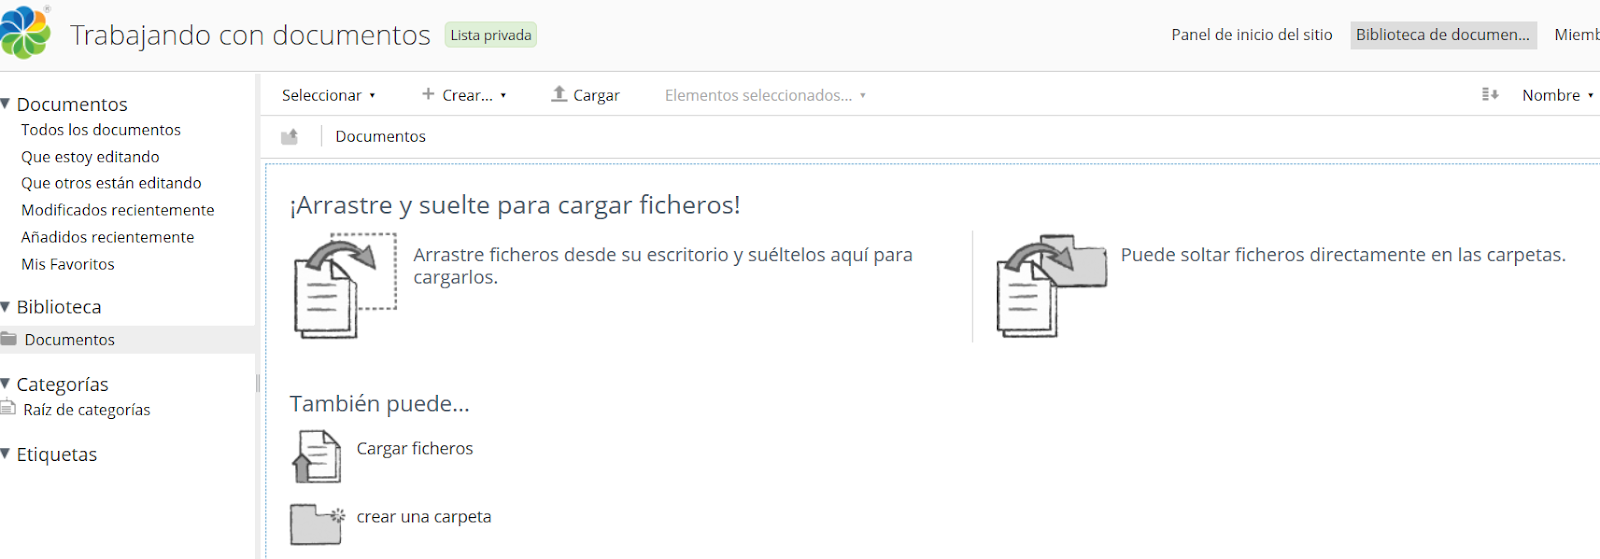
\includegraphics[scale=0.25]{images/files.png}
\end{center}

\begin{center}
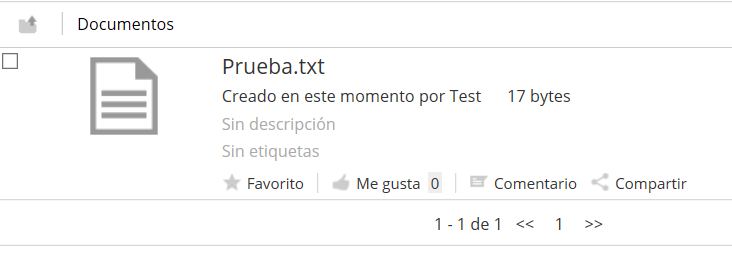
\includegraphics[scale=0.5]{images/file.png}
\end{center}

Y tras cargar el documento correctamente, en el panel principal del espacio de trabajo se pueden comprobar las modificaciones.

\begin{center}
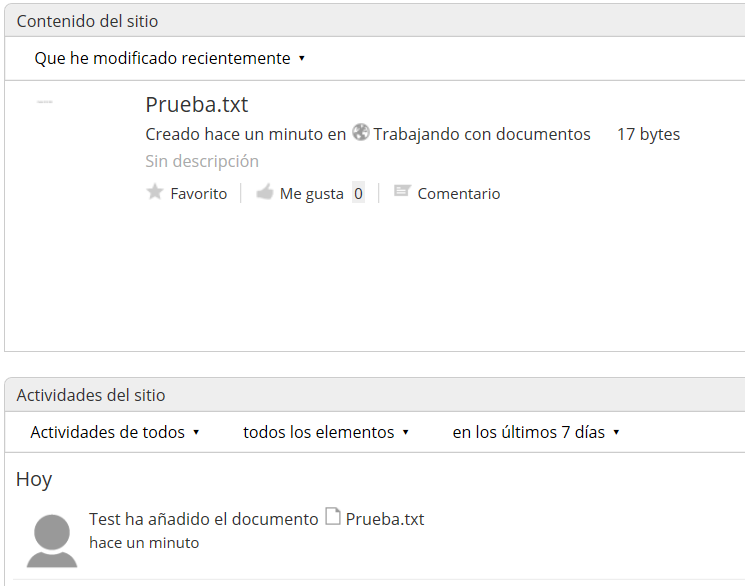
\includegraphics[scale=0.5]{images/mods.png}
\end{center}

Para permitir el versionado del documento subido, hay que administrar los permisos.

\begin{center}
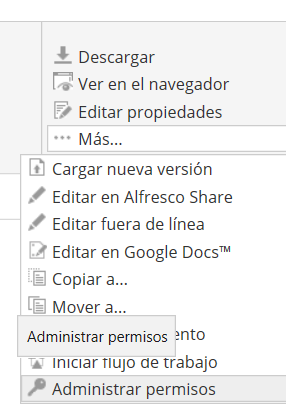
\includegraphics[scale=0.5]{images/ver.png}
\end{center}

Luego se añaden los usuarios y se les asigna un permiso.

\begin{center}
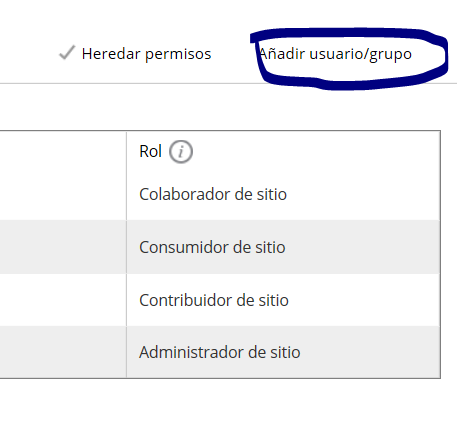
\includegraphics[scale=0.5]{images/permisos.png}
\end{center}

\begin{center}
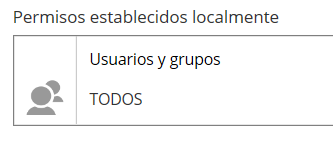
\includegraphics[scale=0.5]{images/permisos2.png}
\end{center}

\begin{center}
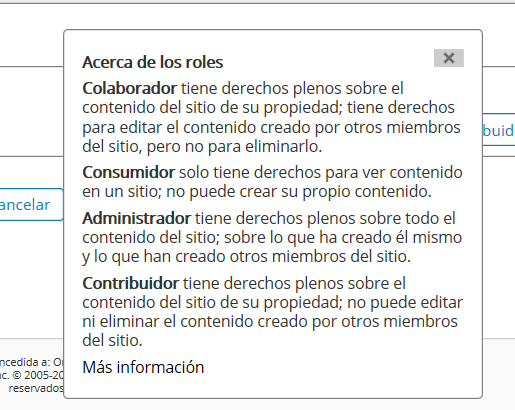
\includegraphics[scale=0.5]{images/info.png}
\end{center}

Se ha añadido el grupo “TODOS”, para que todo el mundo disponga del permiso y se le ha asignado al grupo el rol de “Colaborador”, ya que queremos que todos puedan modificar el documento, derechos sobre el versionado y poder ver el histórico.
Desde otro usuario se ha intentado modificar el documento y se ha podido sin problema.

\begin{center}
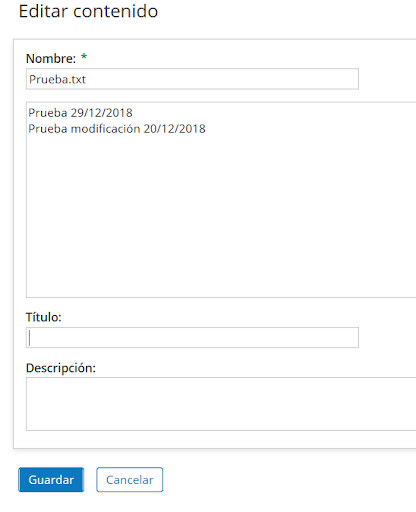
\includegraphics[scale=0.5]{images/mod.png}
\end{center}

\begin{center}
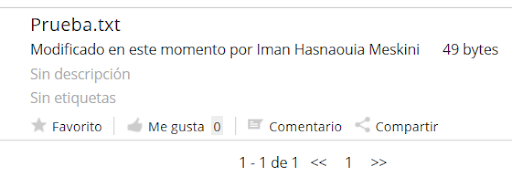
\includegraphics[scale=0.5]{images/mod2.png}
\end{center}

\subsection{Información del histórico de las versiones}

Para probar esta funcionalidad, se ha creado otro archivo .docx para subirlo a la plataforma desde otro usuario que no es Test y crear una nueva versión del documento. Cuando se sube un documento, se muestra toda la información técnica, y hay un apartado en el que se puede especificar la información relativa a la nueva versión. La nueva versión puede tener cambios pequeños o grandes. En este caso, como hemos cambiado el formato del documento y se ha cargado el contenido con varias funcionalidades del editor de documentos, se ha considerado que la nueva versión tiene cambios mayores. Cuando se carga el nuevo fichero, Alfresco cambia automáticamente la versión. Como se puede observar en la imagen, ahora el nombre es Prueba.docx y al lado viene especificada la versión 2.0.

\begin{center}
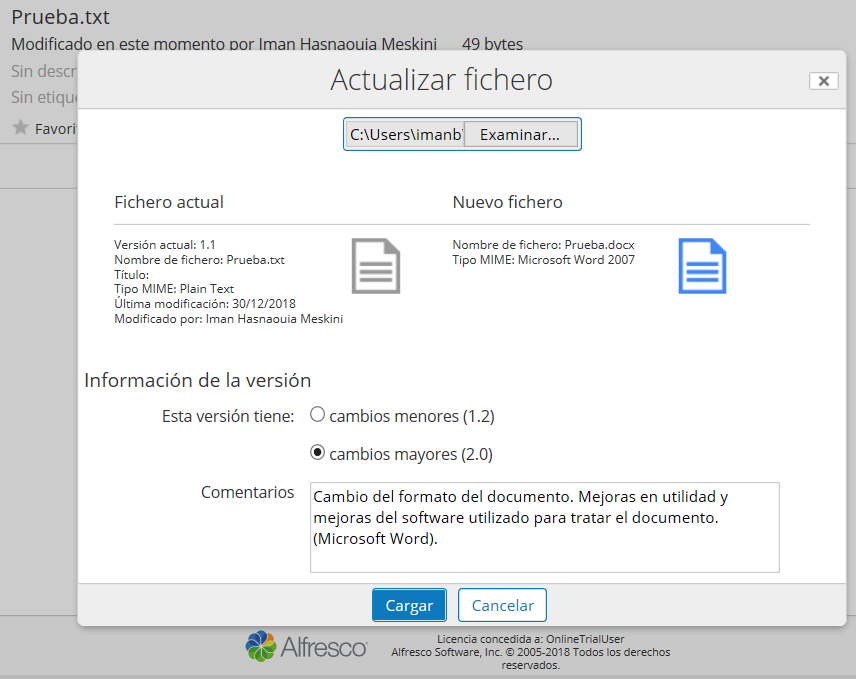
\includegraphics[scale=0.5]{images/actualizacion.png}
\end{center}

\begin{center}
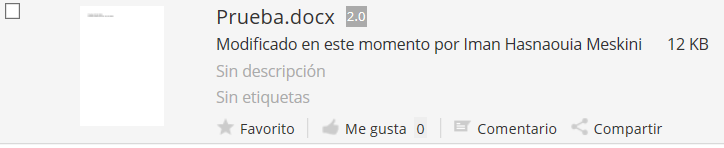
\includegraphics[scale=0.3]{images/version.png}
\end{center}

Cuando se modifica un documento o se sube una nueva versión, se actualiza automáticamente el histórico de versiones. Como se puede observar en la imagen que está debajo cuando se crea o se sube un documento nuevo, la versión es la 1.0. Cuando alguien modifica el documento, la versión sigue siendo la misma, pero se actualiza con una subversión a la 1.1, y por cada modificación se aumenta la subversión 1.2, 1.3, etc. Y cuando se sube una versión nueva específicamente, ya se puede observar que la versión sí cambia a un número mayor, en este caso a la versión 2.0. Si se subiesen más versiones ya sería 3.0, 4.0, etc. Y si se modifica el documento sin modificar la versión, entonces como antes, la versión se actualizaría en el histórico a 2.1, 2.2, 3.1, etc.

\begin{center}
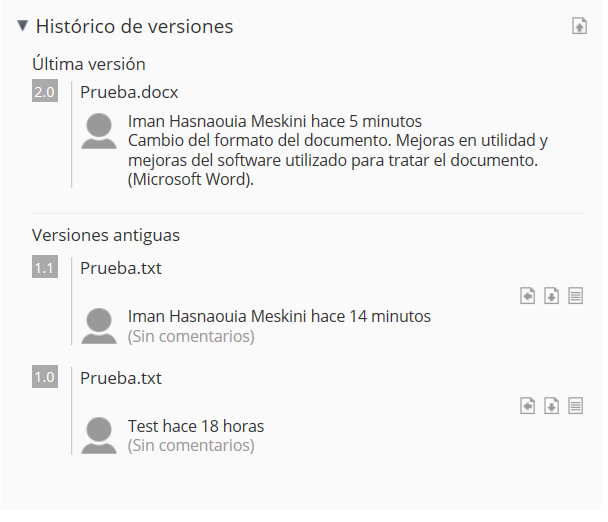
\includegraphics[scale=0.5]{images/versiones.png}
\end{center}

\section{Reglas}

\subsection{Creación de regla de conversión}

Para crear cualquier regla se debe crear una carpeta en la pestaña “Document Library”.  En este caso el nombre de la carpeta es Prueba2.

\begin{center}
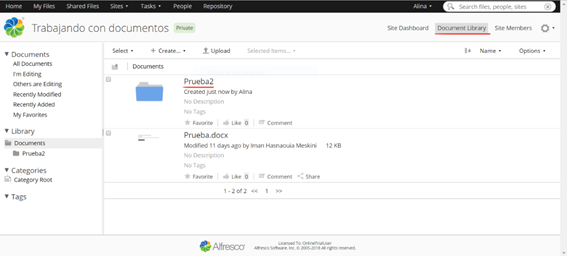
\includegraphics[scale=0.7]{images/regla1.png}
\end{center}

En la carpeta le damos a la sección “More” para desplegar opciones donde aparecerá “Manage Rules”.

\begin{center}
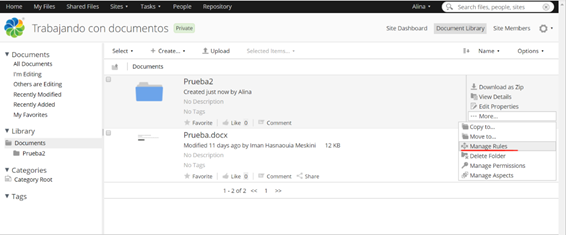
\includegraphics[scale=0.7]{images/regla2.png}
\end{center}

Se abre una sección para crear las reglas donde obligatoriamente le pones el nombre. Si se quiere se pone una descripción para que sea más fácil reconocerla. En nuestro caso, la regla creada es: cuando se alcanza la fecha tope 10/01/2019 (“greater than or equal to”), todos los documentos, tipo Word 2007 creados y modificados en esa carpeta “Prueba2”, serán copiados y guardados también en formato .pdf en la misma carpeta.
A continuación, se describirá cada apartado de la creación de la regla:
\begin{itemize}
\item Nombre: donde es obligatorio
\item Descripción: para facilidad de reconocimiento de regla
\item Cuándo: cuando se vaya a ejecutar la regla, cuando se haya añadido un documento, se haya creado, se haya borrado…
\item Si todos los criterios se cumplen: donde se puede seleccionar criterios como la fecha modificada, el tipo de documento, el autor, tamaño, etc
\item Al menos si se cumple: las mismas opciones que en el apartado de arriba
\end{itemize}
     
\begin{center}
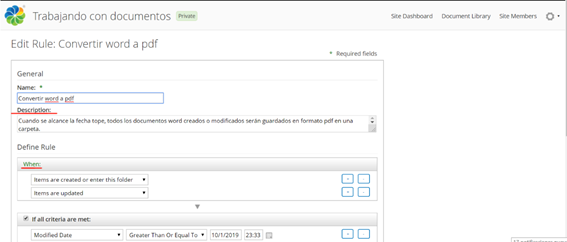
\includegraphics[scale=0.7]{images/regla3.png}
\end{center}

\begin{center}
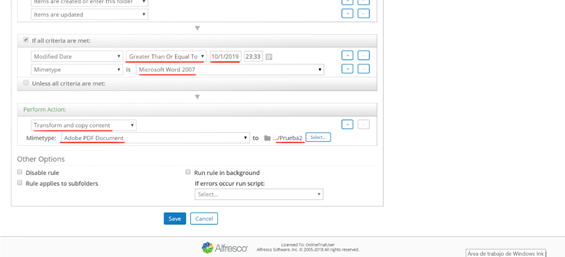
\includegraphics[scale=0.8]{images/regla4.png}
\end{center}

La regla se crea y se guarda y aparece esta pestaña donde se puede ver todas las características de la regla: 

\begin{center}
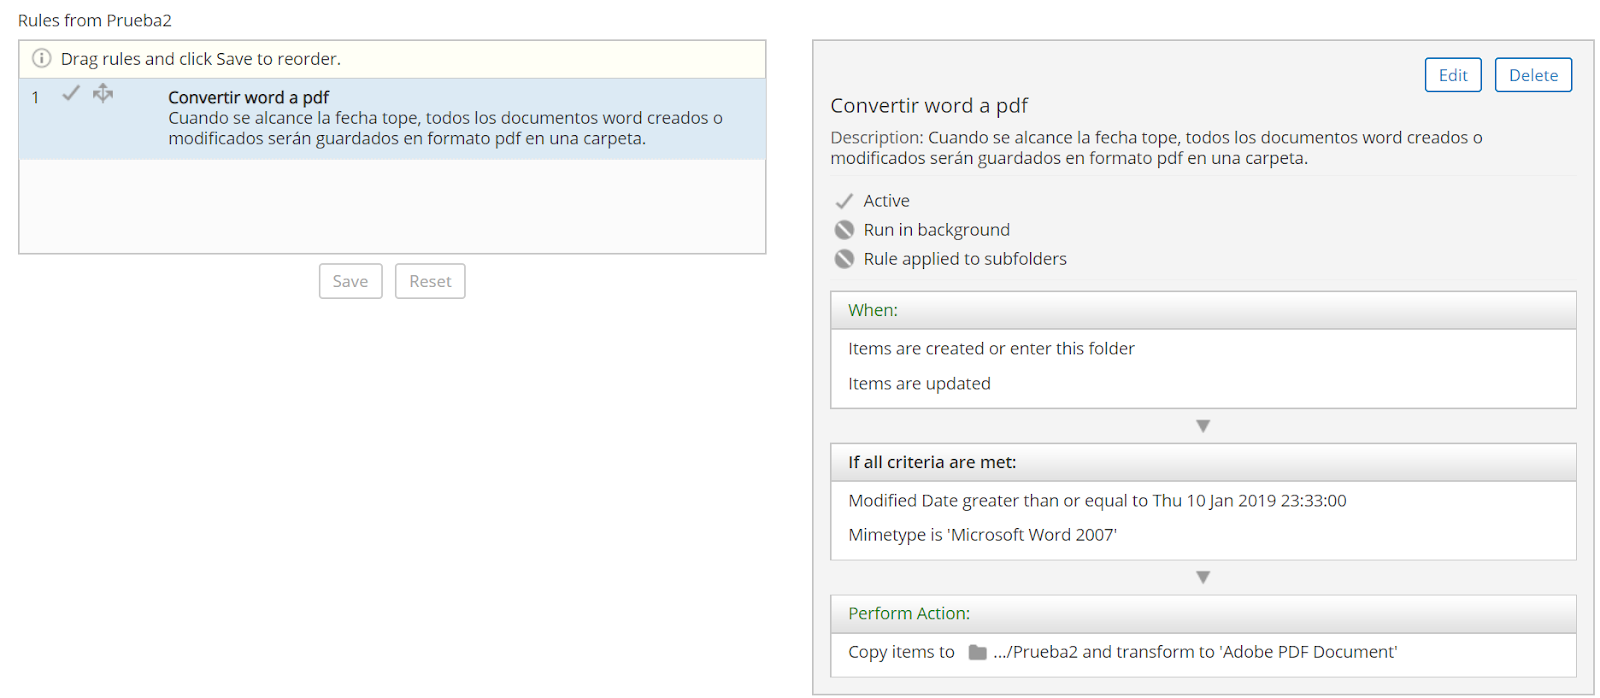
\includegraphics[scale=0.25]{images/regla5.PNG}
\end{center}

\subsection{Probar regla}

Aplicamos la regla y comprobamos si funciona:
Creamos un documento Word y lo guardamos en la carpeta Prueba2, es importante que la fecha de modificación se pase para que se cumpla la regla, en este caso sí ha pasado:

\begin{center}
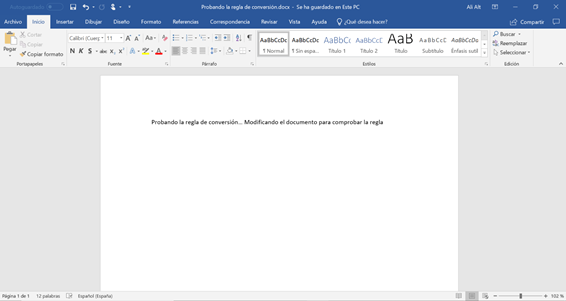
\includegraphics[scale=0.7]{images/word.png}
\end{center}

El documento llamado “Probando la regla de conversión-3” en formato docx que se puede ver abajo ya metido en la carpeta Prueba2.
Vemos que se ha creado con el mismo nombre un documento en formato pdf:

\begin{center}
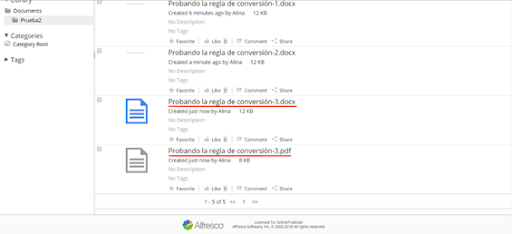
\includegraphics[scale=0.7]{images/pdf.png}
\end{center}

\begin{center}
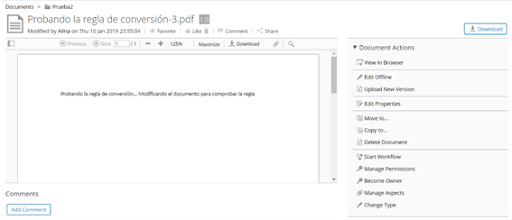
\includegraphics[scale=0.7]{images/conversion.png}
\end{center}

\section{Conclusiones}

\subsection{Conclusiones personales individuales}

\begin{itemize}
\item \textbf{Iman:} La herramienta de Alfresco es bastante útil si la utiliza una organización grande que necesite manejar documentos de manera organizada. Tiene una interfaz de usuario intuitiva, aunque la prueba de primeras es un poco difícil de entender, ya que solamente hay una ventana en la que se pueden subir documentos y crear sitios. Hubiese estado bien que se hubiese especificado que había que utilizar Alfresco Share o cómo utilizar Alfresco en el guion de la práctica, ya que en las documentaciones de otras universidades salen versiones antiguas o versiones que no son online y al principio resulta un poco complicado de entender el uso. Una alternativa más económica sería GitHub, ya que permite compartir y editar documentos, y actualizar versiones, pero esta alternativa sería más viable para un grupo pequeño.
\item \textbf{Alina:} Al realizar la práctica, me he encontrado con algunos problemas, como cuando he querido guardar documento word, (en la herramienta es Microsoft Word) para que se ejecute la regla y lo guarde en pdf. Y tras muchos intentos fallidos, me he dado cuenta de que había que guardar en formato Microsoft Word 2007. Otro problema era que si quería editar un documento word en modo offline, me abría nueva pestaña y me daba error. Todos estos problemas pueden retrasar un proyecto, ya que uno tendría que aprender esos trucos. Y otros problemas técnicas tendría que mejorarlo Alfresco. En general, veo que es una herramienta muy potente y eficiente para las empresas. 
\item \textbf{Cristina:} Alfresco es una aplicación bastante útil e intuitiva, aunque de primeras pueda no parecerlo. En mi parte no me he encontrado ningún problema, ya que en la misma página web de Alfresco explican bastante bien el grado y las formas de integración con otras aplicaciones. Mi opinión personal sobre Alfresco es que, aunque pueda funcionar muy bien en las empresas, considero que GitHub es mucho mejor alternativa, ya que es gratuita, opensource, se puede usar en la aplicación de escritorio, web y línea de comandos y tiene prácticamente las mismas herramientas que GitHub. De hecho, Alfresco tiene su código en GitHub.
\item \textbf{Álvaro:} Alfresco es una herramienta muy potente de cara a la gestión y administración de grandes conjuntos de trabajadores pero, a mi parecer creo que hay mejoras alternativas a esta ya que, aunque la aplicación es bastante intuitiva, tiene varias carencias como el soporte que ofrecen (el 30\% del tiempo útil la plataforma está caída o sobresaturada) y no posee mucha versatilidad en lo que ha lugares para subir ficheros se refiere. Plataformas como GitHub o Trello incluso serían mejores opciones ya que permiten una ordenación más limpia, más visual y una interfaz más agradable y cómoda para el usuario. En resumen, no es una aplicación viable o útil para un conjunto pequeño de personas ni atractivo de cara a un uso continuado debido a su inestable soporte.

\end{itemize}

\subsection{Conclusiones grupales}

En esta práctica hemos probado la funcionalidad de Alfresco Share mediante una versión de prueba. Hemos aprendido a crear un espacio de trabajo, trabajar con documentos de manera compartida observando las múltiples integraciones que tiene Alfresco en relación a los documentos, versionado, etc. También hemos aprendido a usar la funcionalidad de tareas y reglas, asignación de tareas a colaboradores y creación de trabajos de flujo.
Hemos conseguido sacar una idea general de qué es un sistema de gestión documental y cómo usarlo.
Creemos que es una herramienta útil para poder hacer trabajos futuros de la universidad, aunque somos conscientes de que existen varias alternativas a éste y quizás más cómodas de trabajar en entornos de trabajo reducidos. 


\subsection{Relación con teoría}

\begin{itemize}
\item \textbf{Tareas:} Alfresco ofrece una vía para poder estructurar archivos referentes a gestión documental electrónica y transformarlos en archivos electrónicos mediante el proceso de tareas, que serán supervisadas por los colaboradores/administradores del Workflow. Es una herramienta verdaderamente útil en éste sentido, ya que podemos revisar en todo momento que no haya réplicas de archivos (si se resube algún archivo, éste pasará a ser la única versión disponible, la más reciente) y que no haya problemas de múltiples sincronizaciones de edición del archivo ya que los “borradores” serán los únicos documentos que se puedan modificar (el archivo electrónico nunca). Aunque todo esto siempre dependerá de la buena mano y de la subjetividad del buen o mal trabajo que desempeñen cada uno de los revisores de dichos archivos, ya que su toma de decisiones será decisiva para el correcto funcionamiento de los archivos electrónicos.
	
En resumen, las tareas que posee Alfresco da la posibilidad de categorizar, modificar y eliminar archivos de manera simultánea, pero de cara a crear archivos electrónicos estará sujeto al buen trabajo que desempeñen los colaboradores del Workflow para mantener su correcto funcionamiento.

\item \textbf{Gestión de documentos:} Si imaginamos que somos una empresa con múltiples departamentos que necesitan comunicarse entre sí, pero al ser distintos y estar separados la 
comunicación es costosa, la idea de usar un gestor de documentos como Alfresco es llamativa, ya que existe la necesidad de comunicación. Además deque si todos los departamentos utilizan este tipo de plataforma, se normalizaría el formato de los documentos de manera que no habría “islas de información” y la información de cada departamento sería más integrable. Un ejemplo práctico sería la integración con un Sistema de Información de Almacén. El Sistema de Información tiene una base de datos que se va modificando, pero por x razón un departamento necesita toda la información sobre el almacén, por ello, cada cambio implica un documento nuevo, que se podría subir a Alfresco como una nueva versión.
\item \textbf{Reglas:} En una empresa se realizan multitud de acciones repetidas, y el hecho de hacerlas una y otra vez es un gasto de tiempo que se podría invertir en otras cosas. Aparte, otro problema es recordar cumplir esas tareas cuando se haya cumplido una condición, y se podrían olvidarse. Para recordar hacerlas tienes que mirar la lista de tareas, lo que es otra nueva tarea añadida más el tiempo perdido en comprobaciones. Con la regla muchas cosas se simplifican y se automatizan. Ahora es Alfresco quien se va a encargar de realizarlas. Que si necesitas que se cree un documento final en pdf tras el proyecto, se puede hacerlo. Que si se necesita que se notifique a otros colaboradores de una modificación en un documento, pues se les envía un email, o se copian y se mueven documentos de una carpeta a otra, y muchas reglas más que se puedan hacer con esta herramienta para automatizar tareas que tienen ciertas condiciones.  
\item \textbf{Integración:} En nuestra empresa tenemos diferentes departamentos, y cada departamento usa softwares diferentes, que trabajan de forma diferente y producen archivos con diferentes extensiones, y tanto los programas como los archivos tenemos que integrarlos entre sí para que podamos trabajar. Alfresco sirve tanto para almacenar archivos y mantenerlos versionados como para intercambiar información con los programas con los que se integra.

\end{itemize}


\begin{thebibliography}{9}

\bibitem{Tutorial} \textit{Tutorial Alfresco}, \url{http://docs.alfresco.com/6.0/concepts/alfresco-tutorial-02.html}.
\bibitem{Share} \textit{Alfresco Share}, \url{http://www.jpereira.net/attachments/article/50/4-alfresco-Share.pdf}.
\bibitem{Alfresco} \textit{Alfresco}, \url{https://es.wikipedia.org/wiki/Alfresco}.
\bibitem{Integracion} \textit{Extensión e integración de la plataforma Alfresco}, \url{https://www.alfresco.com/es/plataforma/extension-e-integracion-de-alfresco}.

\end{thebibliography}



\end{document}